\section{Виды методов обеспечения качества программного обеспечения}

В этой главе мы рассмотрим некоторые методы обеспечения качества ПО и классифицируем их. Однако перед этим полезно представить себе, что такое обеспечение качества программного обеспечения.

В предыдущей главе мы увидели некоторое количество трактовок определения качества ПО, с точки зрения стандартов, регламентирующих процесс разработки. Обеспечением качества, можно полагать процесс или результат формирования требуемых свойств продукта по мере его создания а также -- поддержания этих свойств по мере внесения изменения в продукт.

Отметим, что это довольно универсальное определение, которое можно применить, как и к обеспечению качества программного обеспечения, так и к обеспечению качества любой другой продукции.

\subsection{Ручные методы}

Ручные методы обеспечения качества программного обеспечения представляют собой с одной стороны, самые простые с точки зрения применения, но, с другой стороны, самые ненадежные способы удостовериться в том, что ПО выполняет возложенные на него задачи. Под ручными методами мы будем понимать все методы, которые не предполагают или не поддаются какой-либо автоматизации.

К таким методам можно отнести, например, код-ревью или тестирование программного обеспечения.

Код-ревью или просмотр кода -- это инженерная практика, заключающаяся в том, что код программы просматривается одним или несколькими разработчиками с целью обнаружения дефектов или же совершенствования навыков разработчика.

Исторически, первым упоминанием код-ревью можно считать работу Майкла Фагана(англ. Michael Fagan) \cite{fagan1999design}, в которой он предлагает методологию нахождения дефектов в программном коде путем его инспекций.

По Фагану, процесс инспекции представляет собой сравнение выхода каждой операции с некоторым выходным критерием. Кроме выходных критериев Фаган вводит входные критерии -- критерии, которым должна удовлетворять операция перед ее началом.

Более подробно, процесс инспекции состоит из следующих операций:

\begin{enumerate}
  \item Планирование(\textit{Planning}). Включает в себя подготовку материалов(кода), места для встречи и встречи участников.
  \item Обзор(\textit{Overview}). Включает ознакомление участников процесса с материалами и назначение ролей.
  \item Подготовка(\textit{Preparation}). Включает непосредственный обзор участниками материалов с целью выяснения возможных дефектов.
  \item Обсуждение(\textit{Inspection meeting}). Включает непосредственное нахождение дефектов.
  \item Исправления(\textit{Rework}). Найденные дефекты исправляются их авторами
  \item Заключение(\textit{Follow-up}). Финальный этап, на котором участники удостоверяются, что все найденные дефекты исправлены и процесс исправлений не породил новых.
\end{enumerate}

\begin{figure}[H]
  \centering
  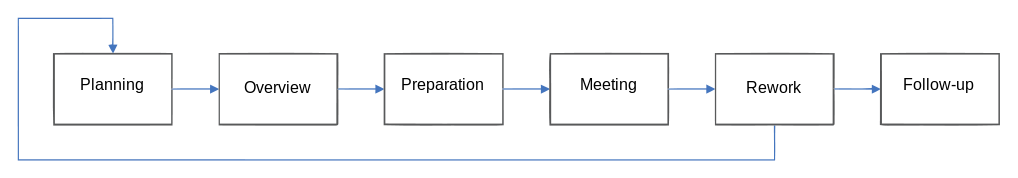
\includegraphics[width=\textwidth]{img/fagan.png}
  \caption{Процесс инспекции кода по Фагану}
\end{figure}

Помимо инспекции кода существует еще и большое количество видов тестирования программного обеспечения. Как-то:

\begin{enumerate}
  \item Функциональное тестирование
  \item Системное тестирование
  \item Тестирование производительности
  \item Регрессионное тестирование
  \item Модульное тестирование
  \item ...
\end{enumerate}

Нас больше интересует так называемое ручное тестирование в ходе которого инженер использует продукт, моделируя действия конечного пользователя. Предыдущие виды тестирования так или иначе используют программные средства для запуска или анализа кода, поэтому его можно отнести скорее к динамическим методам.

Основная идея ручного тестирования заключается в том, что бы посмотреть на систему с точки зрения пользователя и увидеть недостатки в качестве ПО, которые не сразу заметны в ходе разработки. Этот вид тестирования довольно неплохо работает, например, для пользовательских интерфейсов.

Более или менее очевидно, что ручные методы плохо справляются со сложными системами, либо же требуют слишком много времени и усилий. Поэтому далее мы рассмотрим две группы методов, которые используют программные средства и являются более выразительными в том смысле, что позволяют проверить более строгие инварианты в программном коде.

\subsection{Статические методы}

Под статическими методами понимают все методы, которые используют различные артефакты, полученные при проектировании или разработке. Такими артефактами, например, являются требования, спецификации или сам программный код. Важная особенность статических методов заключается в том, что они никоим образом не используют результат выполнения программы. К таки методам относят например, статический анализ кода или формальную верификацию.

Статический анализ кода это процесс выявления ошибок и недочетов в исходном коде, который можно рассматривать как автоматизированный вариант код-ревью. Помимо собственно выявления ошибок, статический анализ позволяет решать задачи рекомендаций по оформлению кода и подсчет метрик кода(например цикломатической сложности или сцепления между двумя программными модулями).

Статические анализаторы обладают тем преимуществом, что позволяют находить огромное количество ошибок еще на этапе программирования, что существенно снижает стоимость их исправления. Кроме того статический анализатор обеспечивает:

\begin{enumerate}
  \item Полное покрытие кода. Участки кода, которые редко получают управление обычно остаются без внимания в ходе код-ревью, между тем являясь потенциальным источником ошибок.
  \item Так как статический анализ не использует результат запуска программы, то он не зависит от окружения, в котором она может исполняться, тем самым позволяя находить ошибки, которые проявляются при смене окружения(компилятора, аппаратной платформы и т. д.)
  \item Не секрет, что человек часто опечатывается по невнимательности и такие ошибки очень сложно обнаружить. Статические анализаторы с легкостью находят ошибки такого рода и позволяют сэкономить огромное количество времени.
\end{enumerate}

Несмотря на кажущуюся современность, история статического анализа кода начинается примерно в 1970-ых годах, с появления утиллиты lint в операционной системе Unix, которая описана в работе Стивена Джонсона(англ. Stephen C. Johnson) \cite{Johnson78lint}. Именно ее можно считать первым статическим анализатором. С современной тоски зрения она была довольно примитивной, но именно она дала начало развитию статических анализаторов.

Формальные методы, в отличии от статического анализа кода, опираются на математический аппарат в ожидании, что его использование существенно повышает надежность разрабатываемой системы. При этом, они довольно сложны и зачастую основываются на не всегда достижимых в реальности предположениях. Формальные методы можно применять на трех уровнях:

\begin{enumerate}
  \item Нулевой. Разрабатывают формальную спецификацию, как артефакт, с оглядкой на который в дальнейшем идет разработка. Очевидно, в этом случае мы все еще не можем гарантировать, что написанный код соответствует спецификации, для чего нужен следующий уровень.
  \item Первый. Программный код \textbf{выводится} из формальной спецификации автоматически, что позволяет неформально рассуждать о том, насколько он соответствует спецификации.
  \item Второй. Полностью формализованные доказательства выводятся и проверяются автоматически.
\end{enumerate}

Формальная верификация занимает первый уровень применения формальных методов. Некоторые конкретные механизмы мы рассмотрим в следующей главе, а здесь же просто скажем, что она собой представляет. Теоретически, основой формальной верификации служит доказательство на некой абстрактной математической модели свойств программной системы в предположении о том, что эта модель адекватно отражает природу вышеозначенной системы. Зачастую для моделирования используют:

\begin{enumerate}
  \item Формальную семантику языка программирования
  \item Теории и типов
  \item Абстрактные автоматы
  \item Вычислительные формализмы, такие как машина Тьюринга или Поста или $\lambda$-исчисление
  \item и т.д.
\end{enumerate}

\subsection{Динамические методы}

К динамическим методам мы отнесем все методы, которые используют результат запуска программы. Основная цель таких методов -- измерить производительность программы в заданных условиях или обнаружить ошибки. Примерами таких методов являются профилирование и тестирование программного обеспечения.

Профилирование представляет собой сбор и измерение характеристик работы программы с целью последующей ее оптимизации. Характеристиками могут выступать время работы программы, используемые ресурсы компьютера, частота вызова определенных функций и так далее. Инструмент, который осуществляет профилирование называется профилировщиком(profiler).

Первым профилировщиком можно считать утиллиту prof из операционной системы Unix, которая занималась тем, что собирала данные о том, сколько времени и с какой частотой происходили вызовы функций в программах, написанных под эту операционную систему. Дальнейшие профилировщики, такие как gprof развивали эту технику, за счет построения и анализа графа вызовов(call graph) функций в программе, что позволяло оценивать насколько часто та или иная функция вызывается относительно других и какое место она занимает в цепочке вызовов. -- \cite{Graham:1982:GCG:872726.806987}.

Современные профилировщики позволяют производить так называемое инструментирование -- модификацию кода программы, с целью сбора данных для анализа. Кроме профилирования, инструментирование полезно в контексте анализа кода в средах разработки.

Тестирование программного обеспечения же, предполагает запуск программы с целью нахождения ошибок. Важным моментом является тот факт, что тестирование именно \textbf{находит} ошибки, в отличии от формальных методов, вкратце описанных раннее, которые \textbf{доказывают} отсутствие ошибок по отношению к спецификации программы. На этот счет широко известна цитата Эдсгера Дейкстры(нидерл. Edsger Wybe Dijkstra) -- <<тестирование показывает не отсутствие ошибок, но их наличие>> из \cite{buxton1970software}.

Мы уже приводили некоторые виды тестирования программного обеспечения в первом разделе этой главы, поэтому не будем повторяться, скажем лишь, что несмотря на кажущуюся ненадежность, тестирование все еще остается одним из самых популярных методов обеспечения качества программного обеспечения, который позволяет убедиться в том, что программа на базовом уровне отвечает требованиям, предъявленным к ней в спецификации.

Многобразие видов тестирования позволяет получать большое количество информации для анализа, а возможность автоматизации позволяет удобно встроить тестирование в жизненный цикл разработки. Например -- автоматический запуск тестов при пересборке прорграммы, что позволяет быстро находить ошибки в программе еще на этапе разработки. 

